\subsection{Properties}
%
\renewcommand{\theequation}{\theenumi}
\begin{enumerate}[label=\arabic*.,ref=\thesubsection.\theenumi]
\numberwithin{equation}{enumi}
%
\item
	Fig. \ref{ch4_circle_def} represents a circle.  The points in the circle are at a distance $r$ from the centre $O$.  $r$ is known as the radius.

\begin{figure}[!ht]
	\begin{center}
		
		%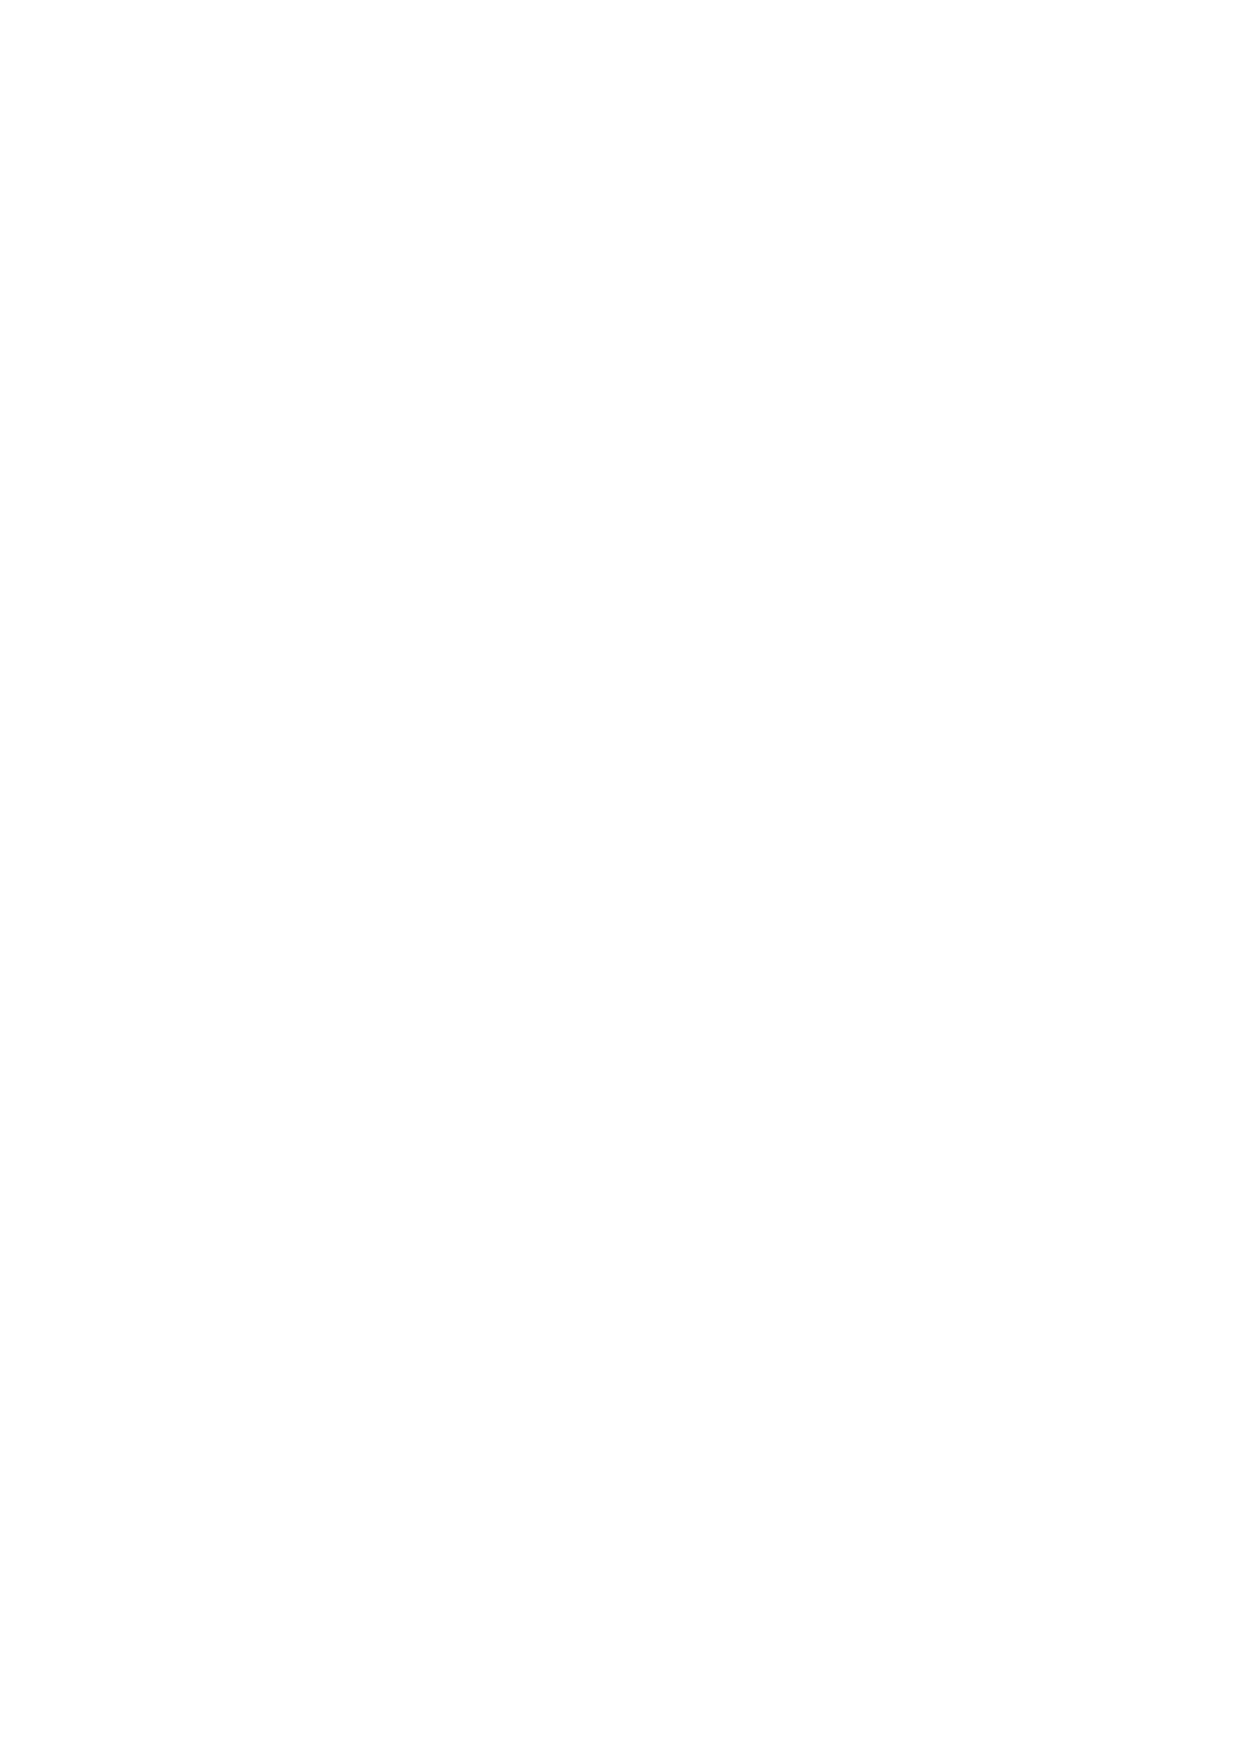
\includegraphics[width=\columnwidth]{./figs/ch4_circle_def}
		%\vspace*{-10cm}
		\resizebox{\columnwidth}{!}{\begin{tikzpicture}
[
scale =3,
>=stealth,
point/.style = {draw, circle, fill = black, inner sep = 1pt},
]
\def\rad{1}
\coordinate [point, label={above : $O$ }] (O) at (0, 0);
\draw (O) circle (\rad);
\node (A) at (-0.7,-0.7)[point,label=above :$A$] {};
\node (B) at (0.7,-0.7)[point,label=above :$B$] {};

\draw (A)--(O);
\draw (O)--(B);
\draw (B)--(A);

\node [above] at (-0.4,-0.4) {$r$};
\node [above] at (0.4,-0.4) {$r$};

\end{tikzpicture}
}
	\end{center}
	\caption{Circle Definitions}
	\label{ch4_circle_def}	
\end{figure}
\item
	In Fig. \ref{ch4_circle_def}, $A$ and $B$ are points on the circle.  The line $AB$ is known as a chord of the circle.

%
%
\item
	\label{ch4_prob_circle_subtend}
	In Fig. \ref{ch4_circle_subtend}  Show that $\angle AOB = 2\angle ACB $.

\begin{figure}[!ht]
	\begin{center}
		
		%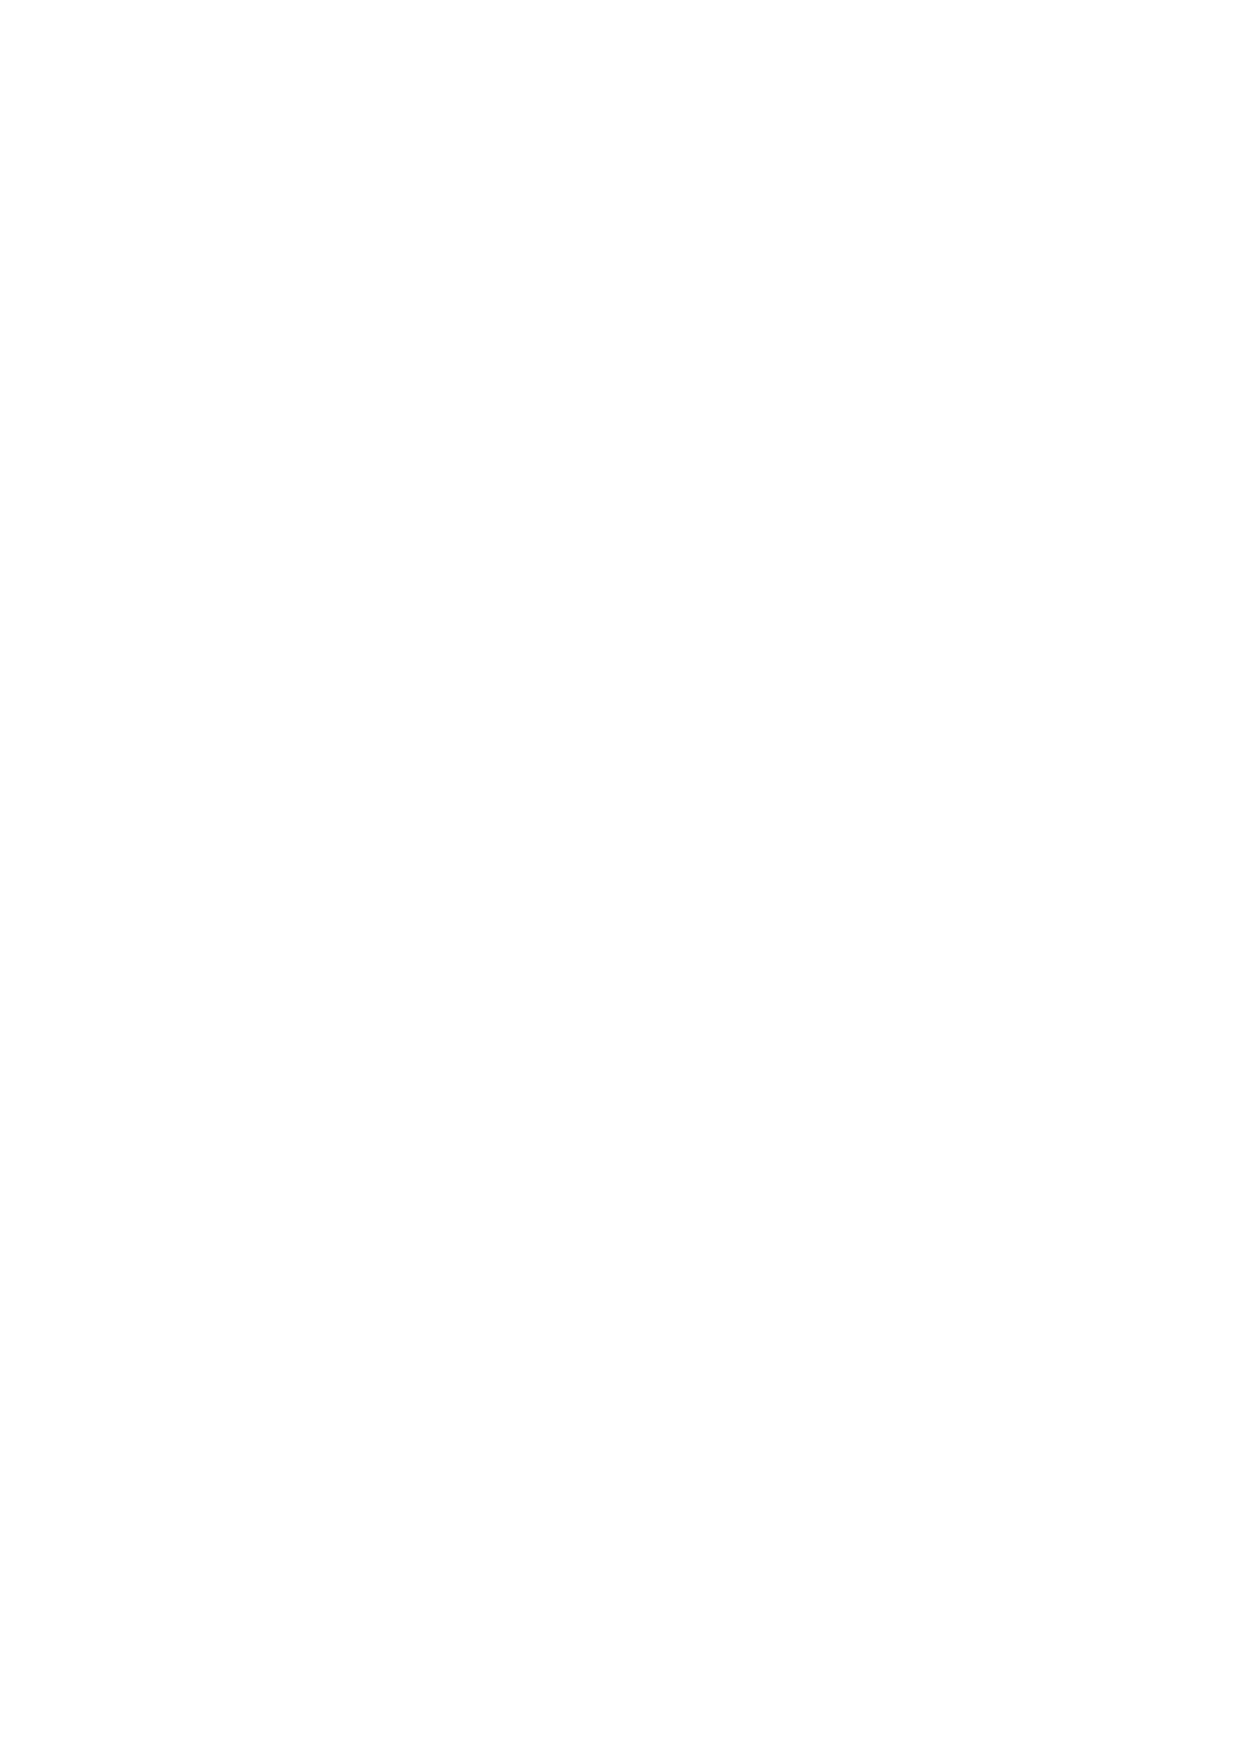
\includegraphics[width=\columnwidth]{./figs/ch4_circle_subtend}
		%\vspace*{-10cm}
		\resizebox{\columnwidth}{!}{\begin{tikzpicture}
[scale =2,>=stealth,point/.style = {draw, circle, fill = black, inner sep = 1pt},]

\def\rad{3}
\coordinate [point, label={above right: $O$ }] (O) at (0, 0);
\draw (O) circle (\rad);
\node (A) at (-2.24,-2)[point,label=below left :$A$] {};
\node (B) at (2.24,-2)[point,label=below right :$B$] {};
\node (C) at (0,3)[point,label=above :$C$] {};
\node (D) at (0,-2)[point,label=below :$D$] {};

\draw (A)--(B);
\draw (B)--(C);
\draw (C)--(A);
\draw (O)--(A);
\draw (O)--(B);
\draw [thick,dashed] (C)--(D);
\tkzMarkAngle[size=0.5](A,C,O)
\tkzMarkAngle[size=0.56](O,C,B)
\tkzMarkAngle[size=0.3](A,O,D)
\tkzMarkAngle[size=0.36](D,O,B)

\draw (-0.1,2.4) node{$\theta_1$};
\draw (0.15,2.3) node{$\theta_2$};

\node [above] at (-0.1,1){$r$};
\node [above] at (-1.1,-1){$r$};
\node [above] at (1.12,-1){$r$};
\node [above] at (-0.2,-0.5){$\alpha$};
\node [above] at (0.2,-0.6){$\beta$};

\end{tikzpicture}
}
	\end{center}
	\caption{Angle subtended by chord $AB$ at the centre $O$ is twice the angle subtended at $P$. }
	\label{ch4_circle_subtend}	
\end{figure}

\solution In Fig. \ref{ch4_circle_subtend}, the triangeles $OPA$ and $OPB$ are isosceles. Hence,
%
\begin{align}
\angle OCA = \angle OAC &= \theta_1 \\
\angle OCB = \angle OBC &= \theta_2
\end{align}
%
Also, $\alpha$ and $\beta$ are exterior angles corresponding to the triangle $AOC$ and $BOC$ respectively. Hence
%
\begin{align}
\alpha &= 2\theta_1 \\
\beta &= 2\theta_2
\end{align}
%
Thus,
%
\begin{align}
\angle AOB &= \alpha + \beta \\
&= 2\brak{\theta_1 + \theta_2} \\
&= 2\angle ACB
\end{align}
%
\item
	The diameter of a circle is the chord that divides the circle into two equal parts. In Fig. \ref{ch4_circle_dia}, $AB$ is the diameter and passes through the centre $O$

%
\item
In Fig. \ref{ch4_circle_dia}, show that $\angle APB = 90^{\degree}$ .

%
\begin{figure}[!ht]
	\begin{center}
		
		%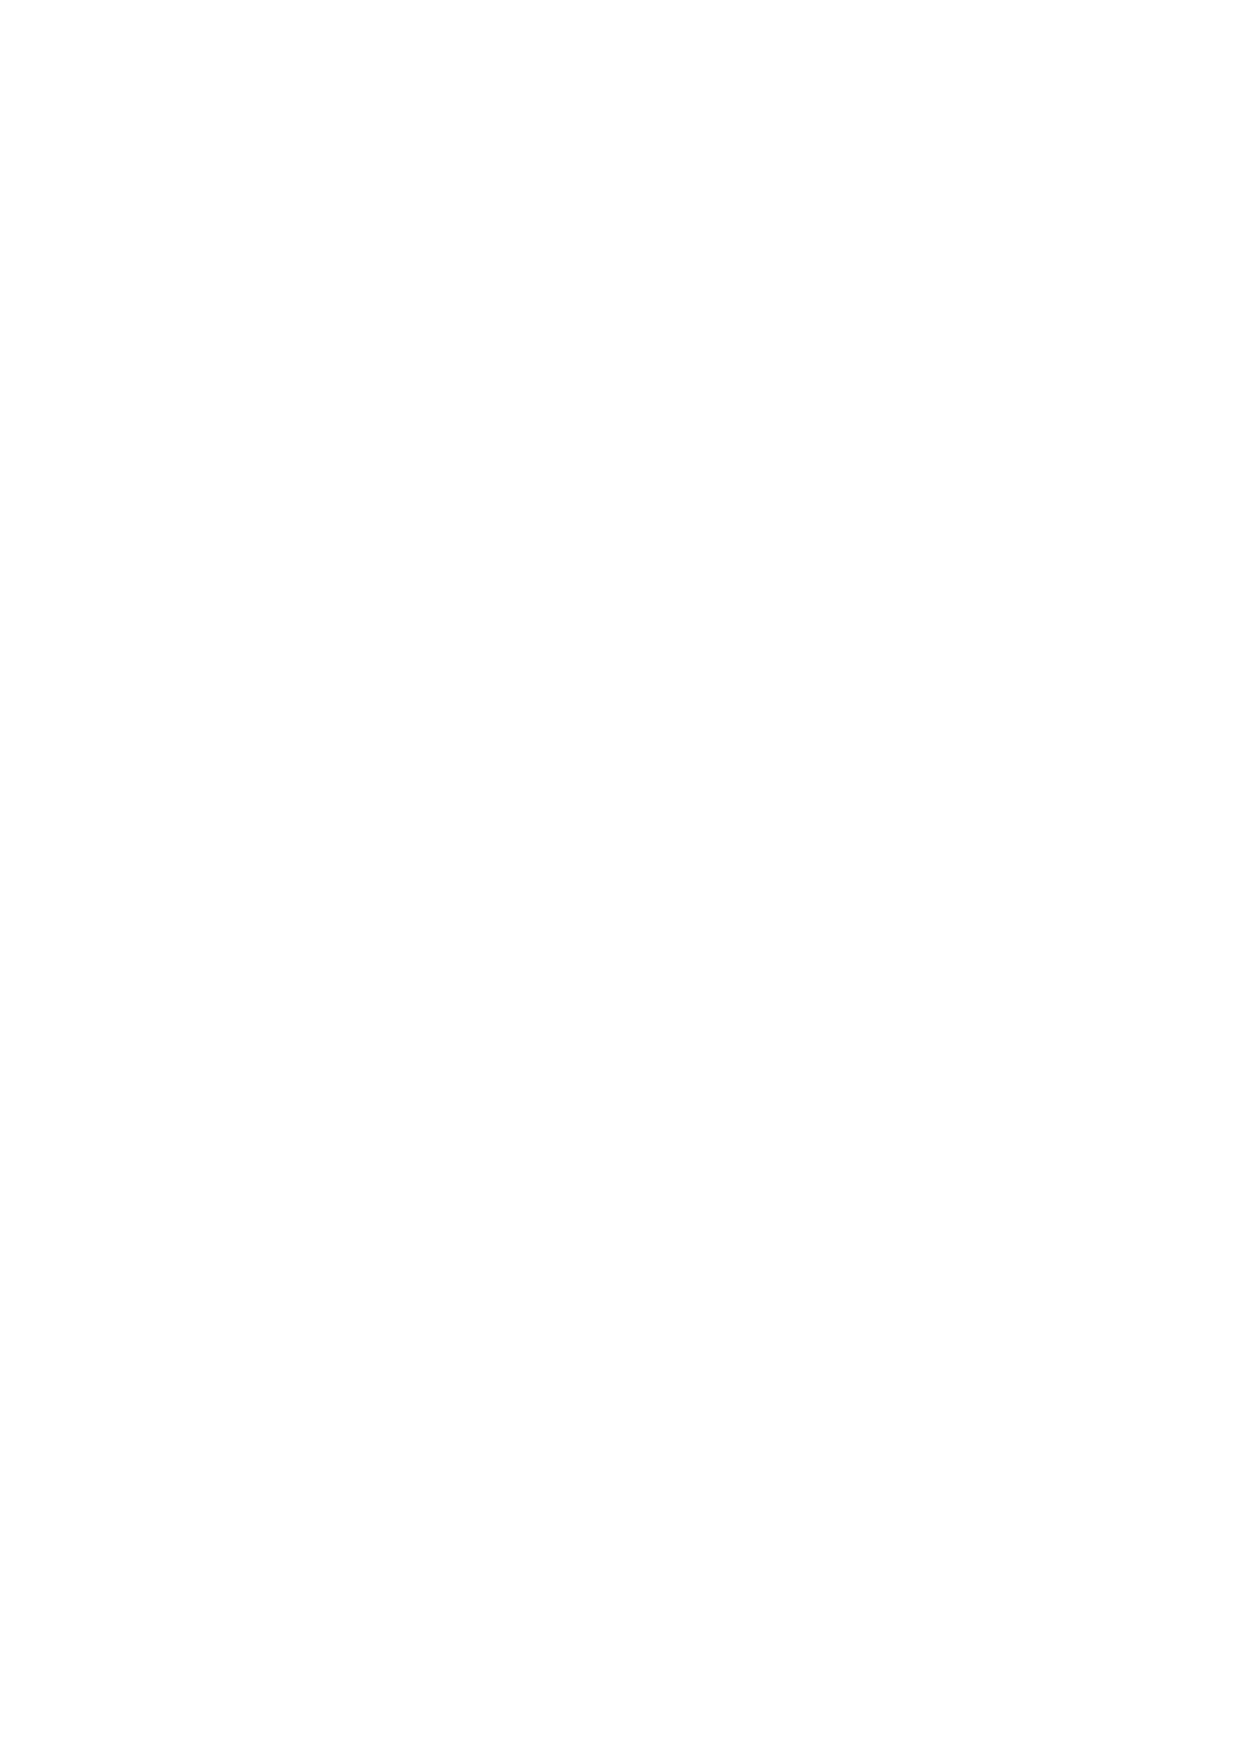
\includegraphics[width=\columnwidth]{./figs/ch4_circle_dia}
		%\vspace*{-10cm}
		\resizebox{\columnwidth}{!}{\begin{tikzpicture}
[scale =3,>=stealth,point/.style = {draw, circle, fill = black, inner sep = 1pt},]

\def\rad{2}
\coordinate [point, label={above : $O$ }] (O) at (0, 0);
\draw (O) circle (\rad);
\node (A) at (-2,0)[point,label=above left :$A$] {};
\node (B) at (2,0)[point,label=above right :$B$] {};
\node (P) at (0,2)[point,label=above :$P$] {};


\draw (A)--(B);
\draw (P)--(A);
\draw (P)--(B);

\tkzMarkRightAngle[size=.2](B,P,A)

\end{tikzpicture}}
	\end{center}
	\caption{Diameter of a circle.}
	\label{ch4_circle_dia}	
\end{figure}
\item
	In Fig. \ref{ch4_chord_product}, show that 
	\begin{equation}
	\begin{split}
\angle ABD &= \angle ACD \\
\angle CAB &= \angle CDB	
	\end{split}
	\end{equation}

\begin{figure}[!ht]
	\begin{center}
		
		%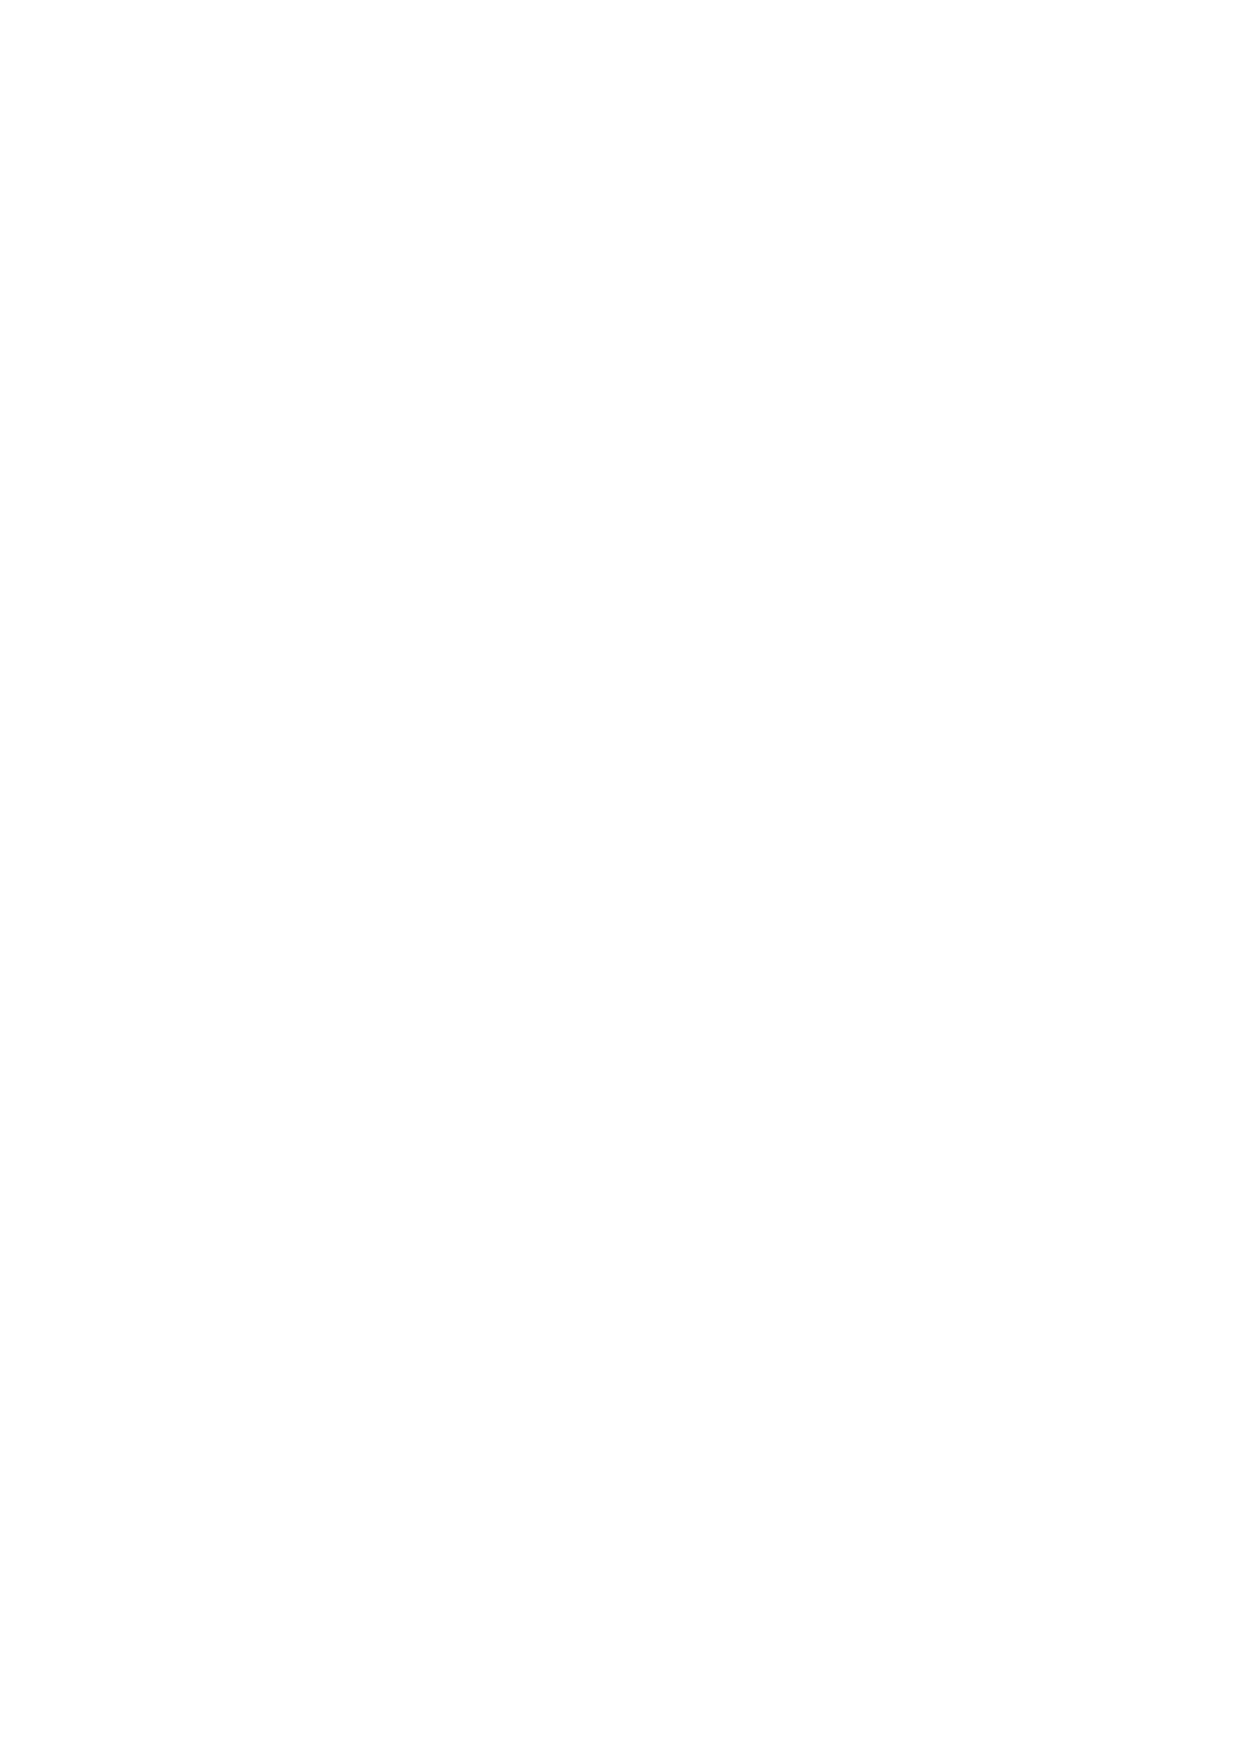
\includegraphics[width=\columnwidth]{./figs/ch4_chord_product}
		%\vspace*{-10cm}
		\resizebox{\columnwidth}{!}{\begin{tikzpicture}
[scale =2,>=stealth,point/.style = {draw, circle, fill = black, inner sep = 1pt},]

\def\rad{3}
\coordinate [point, label={right: $P$ }] (P) at (0, 0);
\draw (P) circle (\rad);
\node (A) at (-2.24,-2)[point,label=below left :$A$] {};
\node (C) at (2.24,-2)[point,label=below right :$C$] {};
\node (B) at (2.24,2)[point,label=above :$B$] {};
\node (D) at (-2.24,2)[point,label=below :$D$] {};

\draw (A)--(B);
\draw (C)--(D);
\draw [thick,dashed] (A)--(C);
\draw [thick,dashed] (B)--(D);
\tkzMarkAngle[size=0.3](P,D,B)
\tkzMarkAngle[size=0.3](D,B,P)
\tkzMarkAngle[size=0.3](B,P,D)
\tkzMarkAngle[size=0.3](A,P,C)
\tkzMarkAngle[size=0.3](C,A,P)
\tkzMarkAngle[size=0.3](P,C,A)

\draw (1.8,1.8) node{$\alpha$};
\draw (-1.84,1.84) node{$\beta$};
\draw (-1.8,-1.9) node{$\beta$};
\draw (1.8,-1.9) node{$\alpha$};
\draw (0,0.4) node{$\theta$};
\draw (0,-0.4) node{$\theta$};

\end{tikzpicture}}
	\end{center}
	\caption{$PA.PB = PC.PD$}
	\label{ch4_chord_product}	
\end{figure}
%
%
\solution Use Problem \ref{ch4_prob_circle_subtend}.
%
\item
	In Fig. \ref{ch4_chord_product}, show that the triangles $PAB$ and $PBD$ are similar

\solution Trivial using previous problem
\item
	In Fig. \ref{ch4_chord_product}, show that 
	\begin{equation}
	PA.PB = PC.PD
	\end{equation}

%
\solution Since triangles $PAC$ and $PBD$ are similar, 
%
\begin{align}
\frac{PA}{PD} &= \frac{PC}{PB} \\
\Rightarrow PA.PB &= PC.PD
\end{align}
%
%
\item
	Show that 
	\begin{equation}
	\label{ch5_sin_zero}
	\sin 0^{\degree} = 0
	\end{equation}

\solution From \eqref{ch1_trig_defs}, $\theta \to 0\degree \implies a \to 0 \implies \sin \theta $ and %
\item
	Show that 
	\begin{equation}
	\label{ch5_cos_zero}
	\cos 0^{\degree} = 1
	\end{equation}

\solution Follows from the fact that $\sin 0 = 0$ and \eqref{eq:tri_sin_cos_id}.
% 	
\item
	Show that 
	\begin{equation}
	\label{ch5_cos_90}
	\cos 90^{\degree} = 0
	\end{equation}

\solution Follows from the fact that $\cos 90 \degree = \sin \brak{90\degree -90\degree} = 0$ using \eqref{eq:tri_90-ang}.
\item
	The line $PX$ in Fig. \ref{ch4_tangent_def} touches the circle at exactly one  point $P$. It is known as the tangent to the circle.
%
%
\item
	Show that $OP \perp PX$.
% is the perpendicular to the line $PX$ as shown in the Fig. \ref{ch4_short_dist}. Show that $OP$ is the shortest distance between the point $O$ and the line $PX$. 

\solution Without loss of generality, let $0 \le \theta \le 90^{\degree}$. Using the cosine formula in $\triangle OPP_n$,\begin{align}
\brak{r+d_n}^2 > r^2,
\end{align}
%Let $P_1$ be a point on the line $PX$. Then $OPP_1$ is a right angled triangle.  Using Budhayana's theorem,
%
\begin{figure}[!ht]
	\begin{center}
		
		%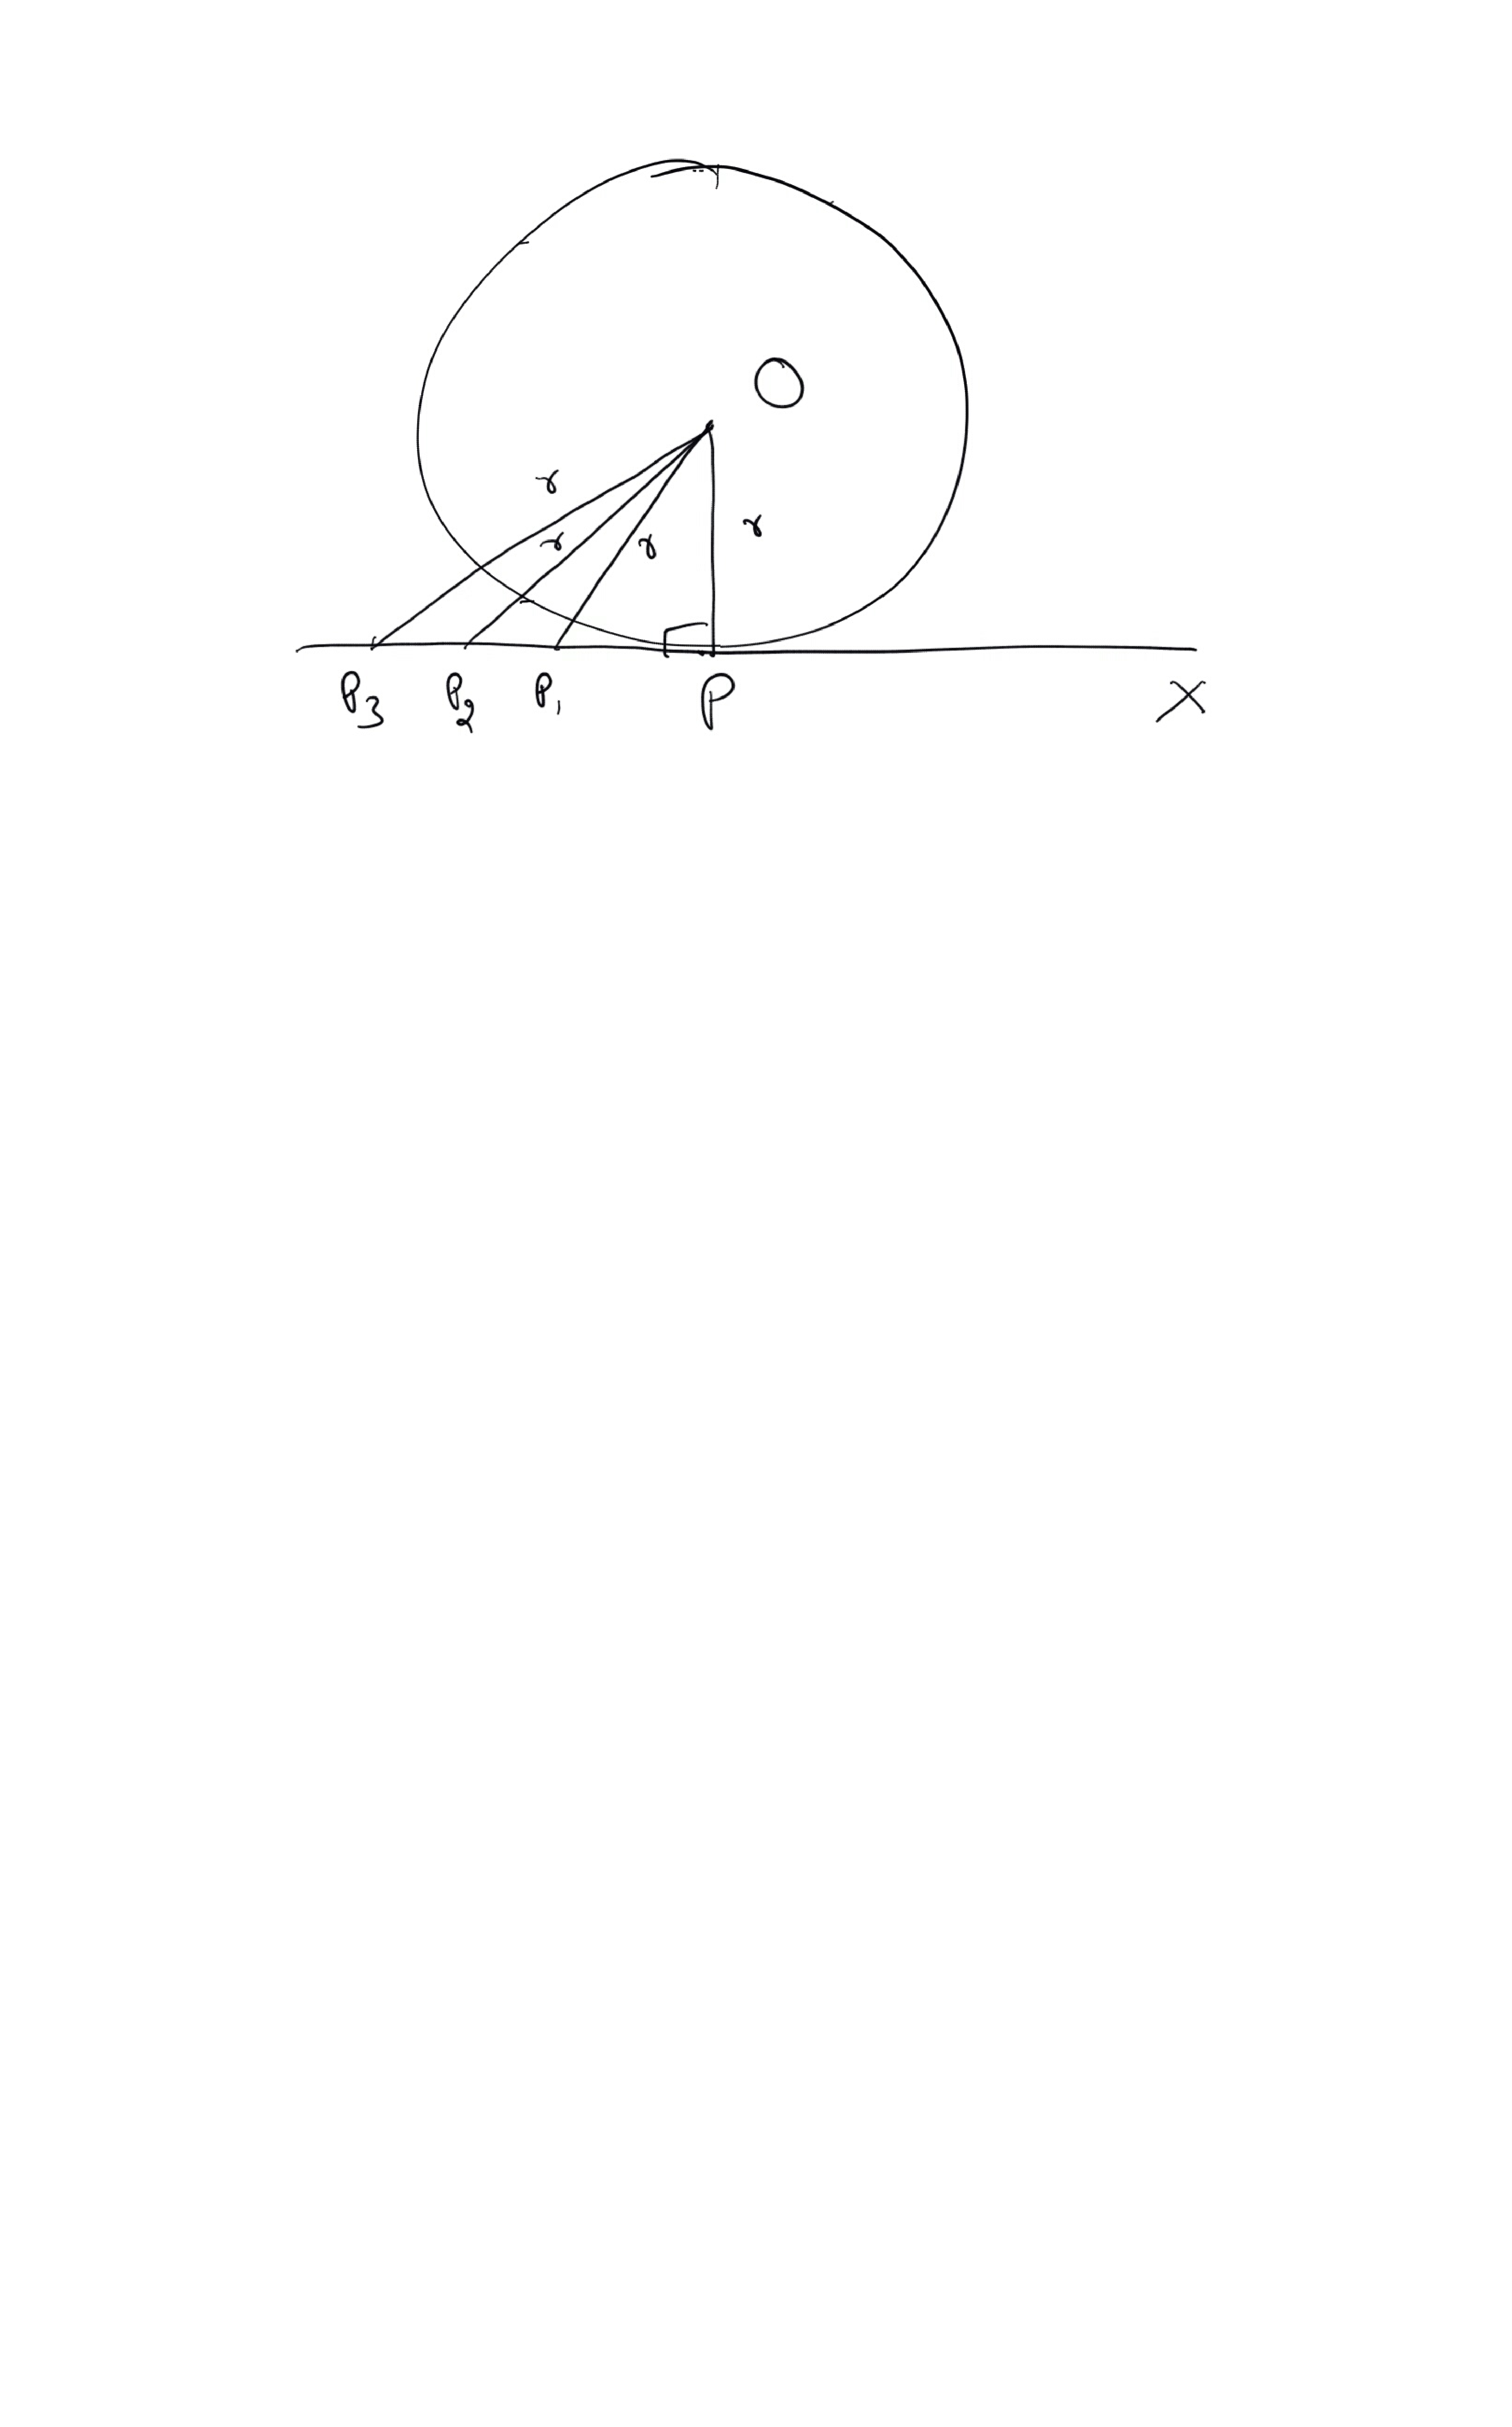
\includegraphics[width=\columnwidth]{./figs/ch4_tangent_def}
		%\vspace*{-10cm}
		\resizebox{\columnwidth}{!}{\begin{tikzpicture}
[scale =2,>=stealth,point/.style = {draw, circle, fill = black, inner sep = 1pt},]

\def\rad{2}
\coordinate [point, label={right: $O$ }] (O) at (0, 2);
\draw (O) circle (\rad);
\node (P) at (0,0)[point,label=below :$P$] {};
\node (X) at (2,0)[point,label=right :$X$] {};
\node (Y) at (-4,0)[point,label=left :$Y$] {};
\node (P_1) at (-1,0)[point,label=below  :$P_1$] {};
\node (P_2) at (-2,0)[point,label=below  :$P_2$] {};
\node (P_3) at (-3,0)[point,label=below  :$P_3$] {};

\draw (O)--(P);
\draw (X)--(Y);
\draw (O)--(P_1);
\draw (O)--(P_2);
\draw (O)--(P_3);

\tkzMarkRightAngle[size=.2](O,P,P_1);
\node [above] at (-0.8,0.5){$r$};
\node [above] at (-1.2,0.8){$r$};
\node [above] at (-1.45,1){$r$};
\node [above] at (0.1,0.8){$r$};
\end{tikzpicture}}
	\end{center}
	\caption{Tangent to a Circle.}
	\label{ch4_tangent_def}	
\end{figure}
%
%\begin{figure}[!ht]
%	\begin{center}
%		
%		%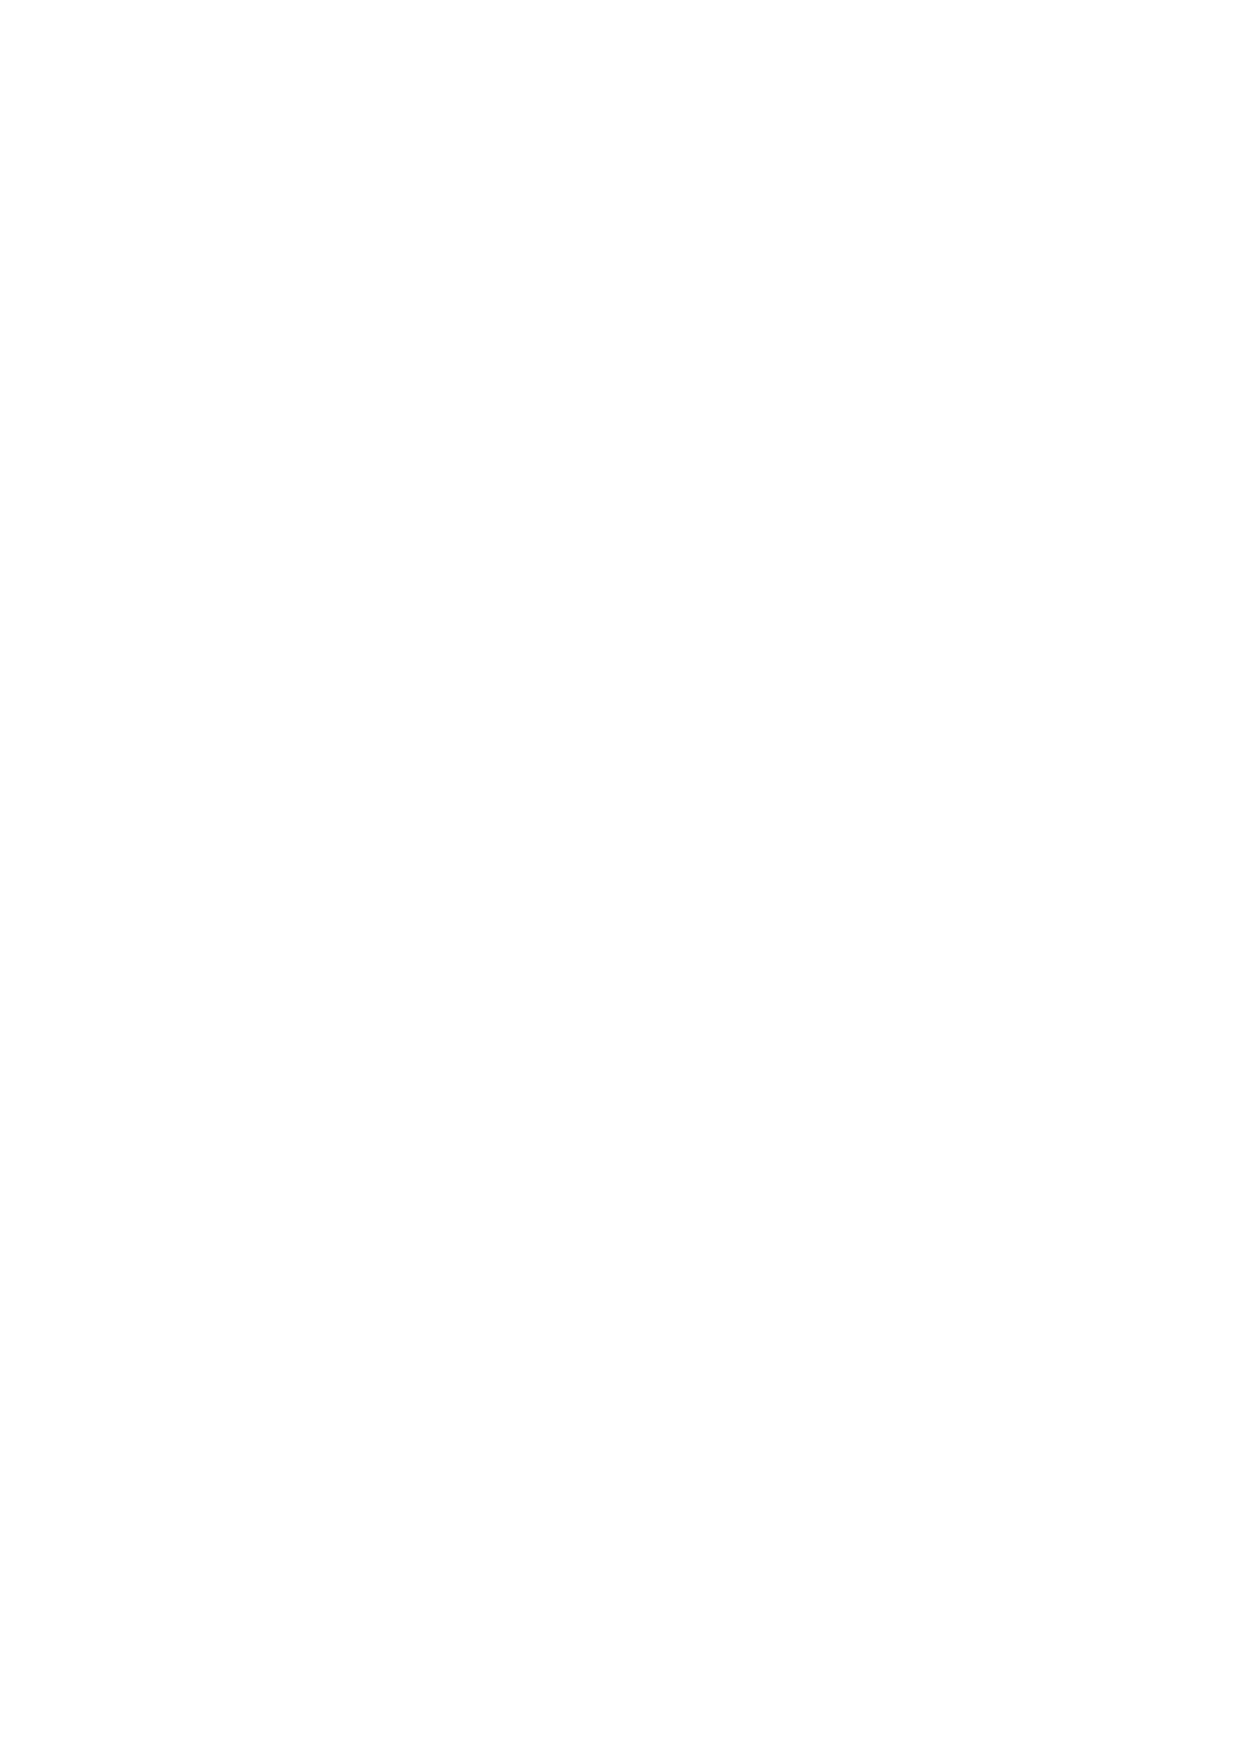
\includegraphics[width=\columnwidth]{./figs/ch4_short_dist}
%		%\vspace*{-10cm}
%		\resizebox{\columnwidth}{!}{\begin{tikzpicture}
[scale =2,>=stealth,point/.style = {draw, circle, fill = black, inner sep = 1pt},]


\node (O) at (0,3)[point,label=above :$O$] {};
\node (P) at (0,0)[point,label=below :$P$] {};
\node (P_1) at (-1.5,0)[point,label=below :$P_1$] {};
\node (P_2) at (-3,0)[point,label=below :$P_2$] {};
\node (X) at (2,0)[point,label=right :$X$] {};
\node (Y) at (-4,0)[point,label=left :$Y$] {};
\draw (O)--(P);
\draw (X)--(Y);
\draw (O)--(P_1);
\draw (O)--(P_2);

\tkzMarkRightAngle[size=.2](O,P,X);

\end{tikzpicture}}
%	\end{center}
%	\caption{Shortest distance from $O$ to line $PX$}
%	\label{ch4_short_dist}	
%\end{figure}

%
\begin{align}
%\begin{split}
\brak{r+d_n}^2 = r^2 + x_n^2 - 2rx_n\cos\theta > r^2 
\\
\implies  0 <\cos\theta < \frac{x_n}{2r},
%OP_1^2 &= OP^2 + PP_1^2 \\
%\Rightarrow OP_1 > OP
%\end{split}
\end{align}
%
where $x_n$ can be made as small as we choose.  Thus, 
%
\begin{align}
\cos \theta = 0 \implies \theta  = 90 ^{\degree}.
\end{align}

%\solution In Fig. \ref{ch4_tangent_def}, we can see that $OP$ is is the radius of the circle and the length of all line segments from $O$ to the line $PX > r$.  Using the result of the previous 
%problem, it is obvious that $OP \perp PX$. 
%
	%
\item
In Fig. \ref{ch4_tangent_prod} show that 
%
\begin{equation}
\angle PCA = \angle PBC
\end{equation}
%
$O$ is the centre of the circle and $PC$ is the tangent.

	\begin{figure}[!ht]
		\begin{center}
			
			%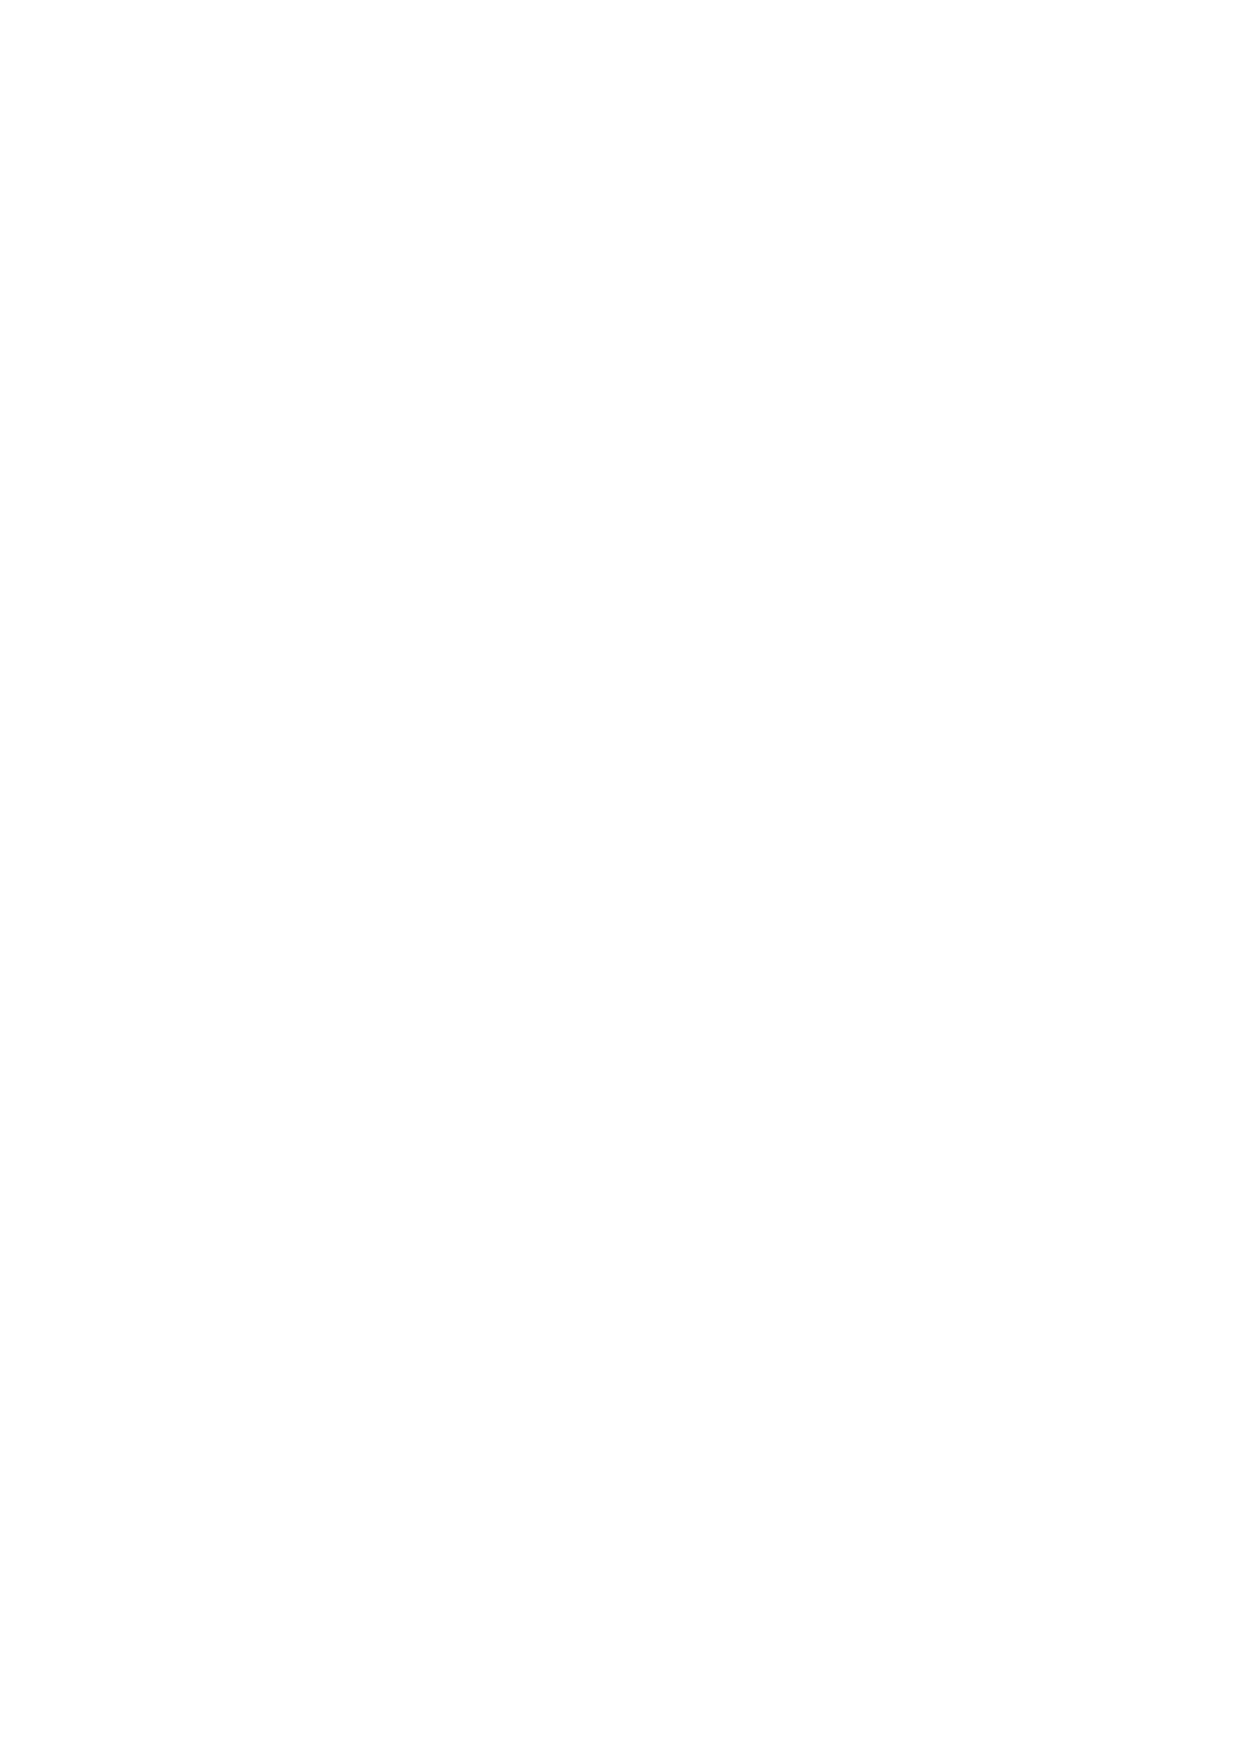
\includegraphics[width=\columnwidth]{./figs/ch4_tangent_prod}
			%\vspace*{-10cm}
			\resizebox{\columnwidth}{!}{\begin{tikzpicture}
[scale =2,>=stealth,point/.style = {draw, circle, fill = black, inner sep = 1pt},]

\def\rad{2}
\coordinate [point, label={above: $O$ }] (O) at (0, 2);
\draw (O) circle (\rad);
\node (P) at (-4,0)[point,label=below :$P$] {};
\node (C) at (0,0)[point,label=below :$C$] {};
\node (A) at (-1.92,1.45)[point,label=above left :$A$] {};
\node (B) at (1.2,3.6)[point,label=above right :$B$] {};
\draw (O)--(C);
\draw (P)--(C);
\draw (P)--(B);
\draw (A)--(C);
\draw (B)--(C);

\draw [thick,dashed](A)--(O);
\tkzMarkRightAngle[size=.2](P,C,O);
\tkzMarkAngle[size=.3](A,B,C);
\tkzMarkAngle[size=.4](O,C,A);
%\tkzMarkAngle[size=.5](B,C,O);
%\tkzMarkAngle[size=.3](P,A,C);
\tkzMarkAngle[size=.2](C,A,O);
\tkzMarkAngle[size=.2](A,O,C);

\node [above] at (0.65,1.5){$r$};
\node [above] at (-0.9,1.7){$r$};
\node [above] at (0.1,1){$r$};
%\draw (-1.9,1) node{$\theta$};

\draw (0.95,3.3) node{$\alpha$};
\draw (-0.2,1.7) node{$2\alpha$};
\draw (-0.2,0.5) node{$90-\alpha$};
\draw (-1.4,1.4) node{$90-\alpha$};
%\draw (.1,.6) node{$\phi$};

\end{tikzpicture}}
		\end{center}
		\caption{$PA.PB = PC^2$.}
		\label{ch4_tangent_prod}	
	\end{figure}
	%

%
\solution Obvious from the figure once we observe that $\triangle OAC$ is isosceles.
%
%
\item
	In Fig. \ref{ch4_tangent_prod}, show that the triangles $PAC$ and $PBC$ are similar.

\solution From the previous problem, it is obvious that corresponding angles of both triangles are equal.  Hence they are similar.
%
\item
	Show that $PA.PB = PC^2$

\solution Since $\Delta PAC \sim \Delta PBC$, their sides are in the same ratio.  Hence,
%
\begin{align}
\frac{PA}{PC} &= \frac{PC}{PB} \\
\Rightarrow PA.PB &=PC^2
\end{align}
%
\item
Given that $PA.PB = PC^2$, show that $PC$ is a tangent to the circle.

%
\item
	In Fig. \ref{ch4_chord_tangent_prod}, show that\begin{equation}
	PA.PB = PC.PD
	\end{equation}

%
\begin{figure}[!ht]
	\begin{center}
		
		%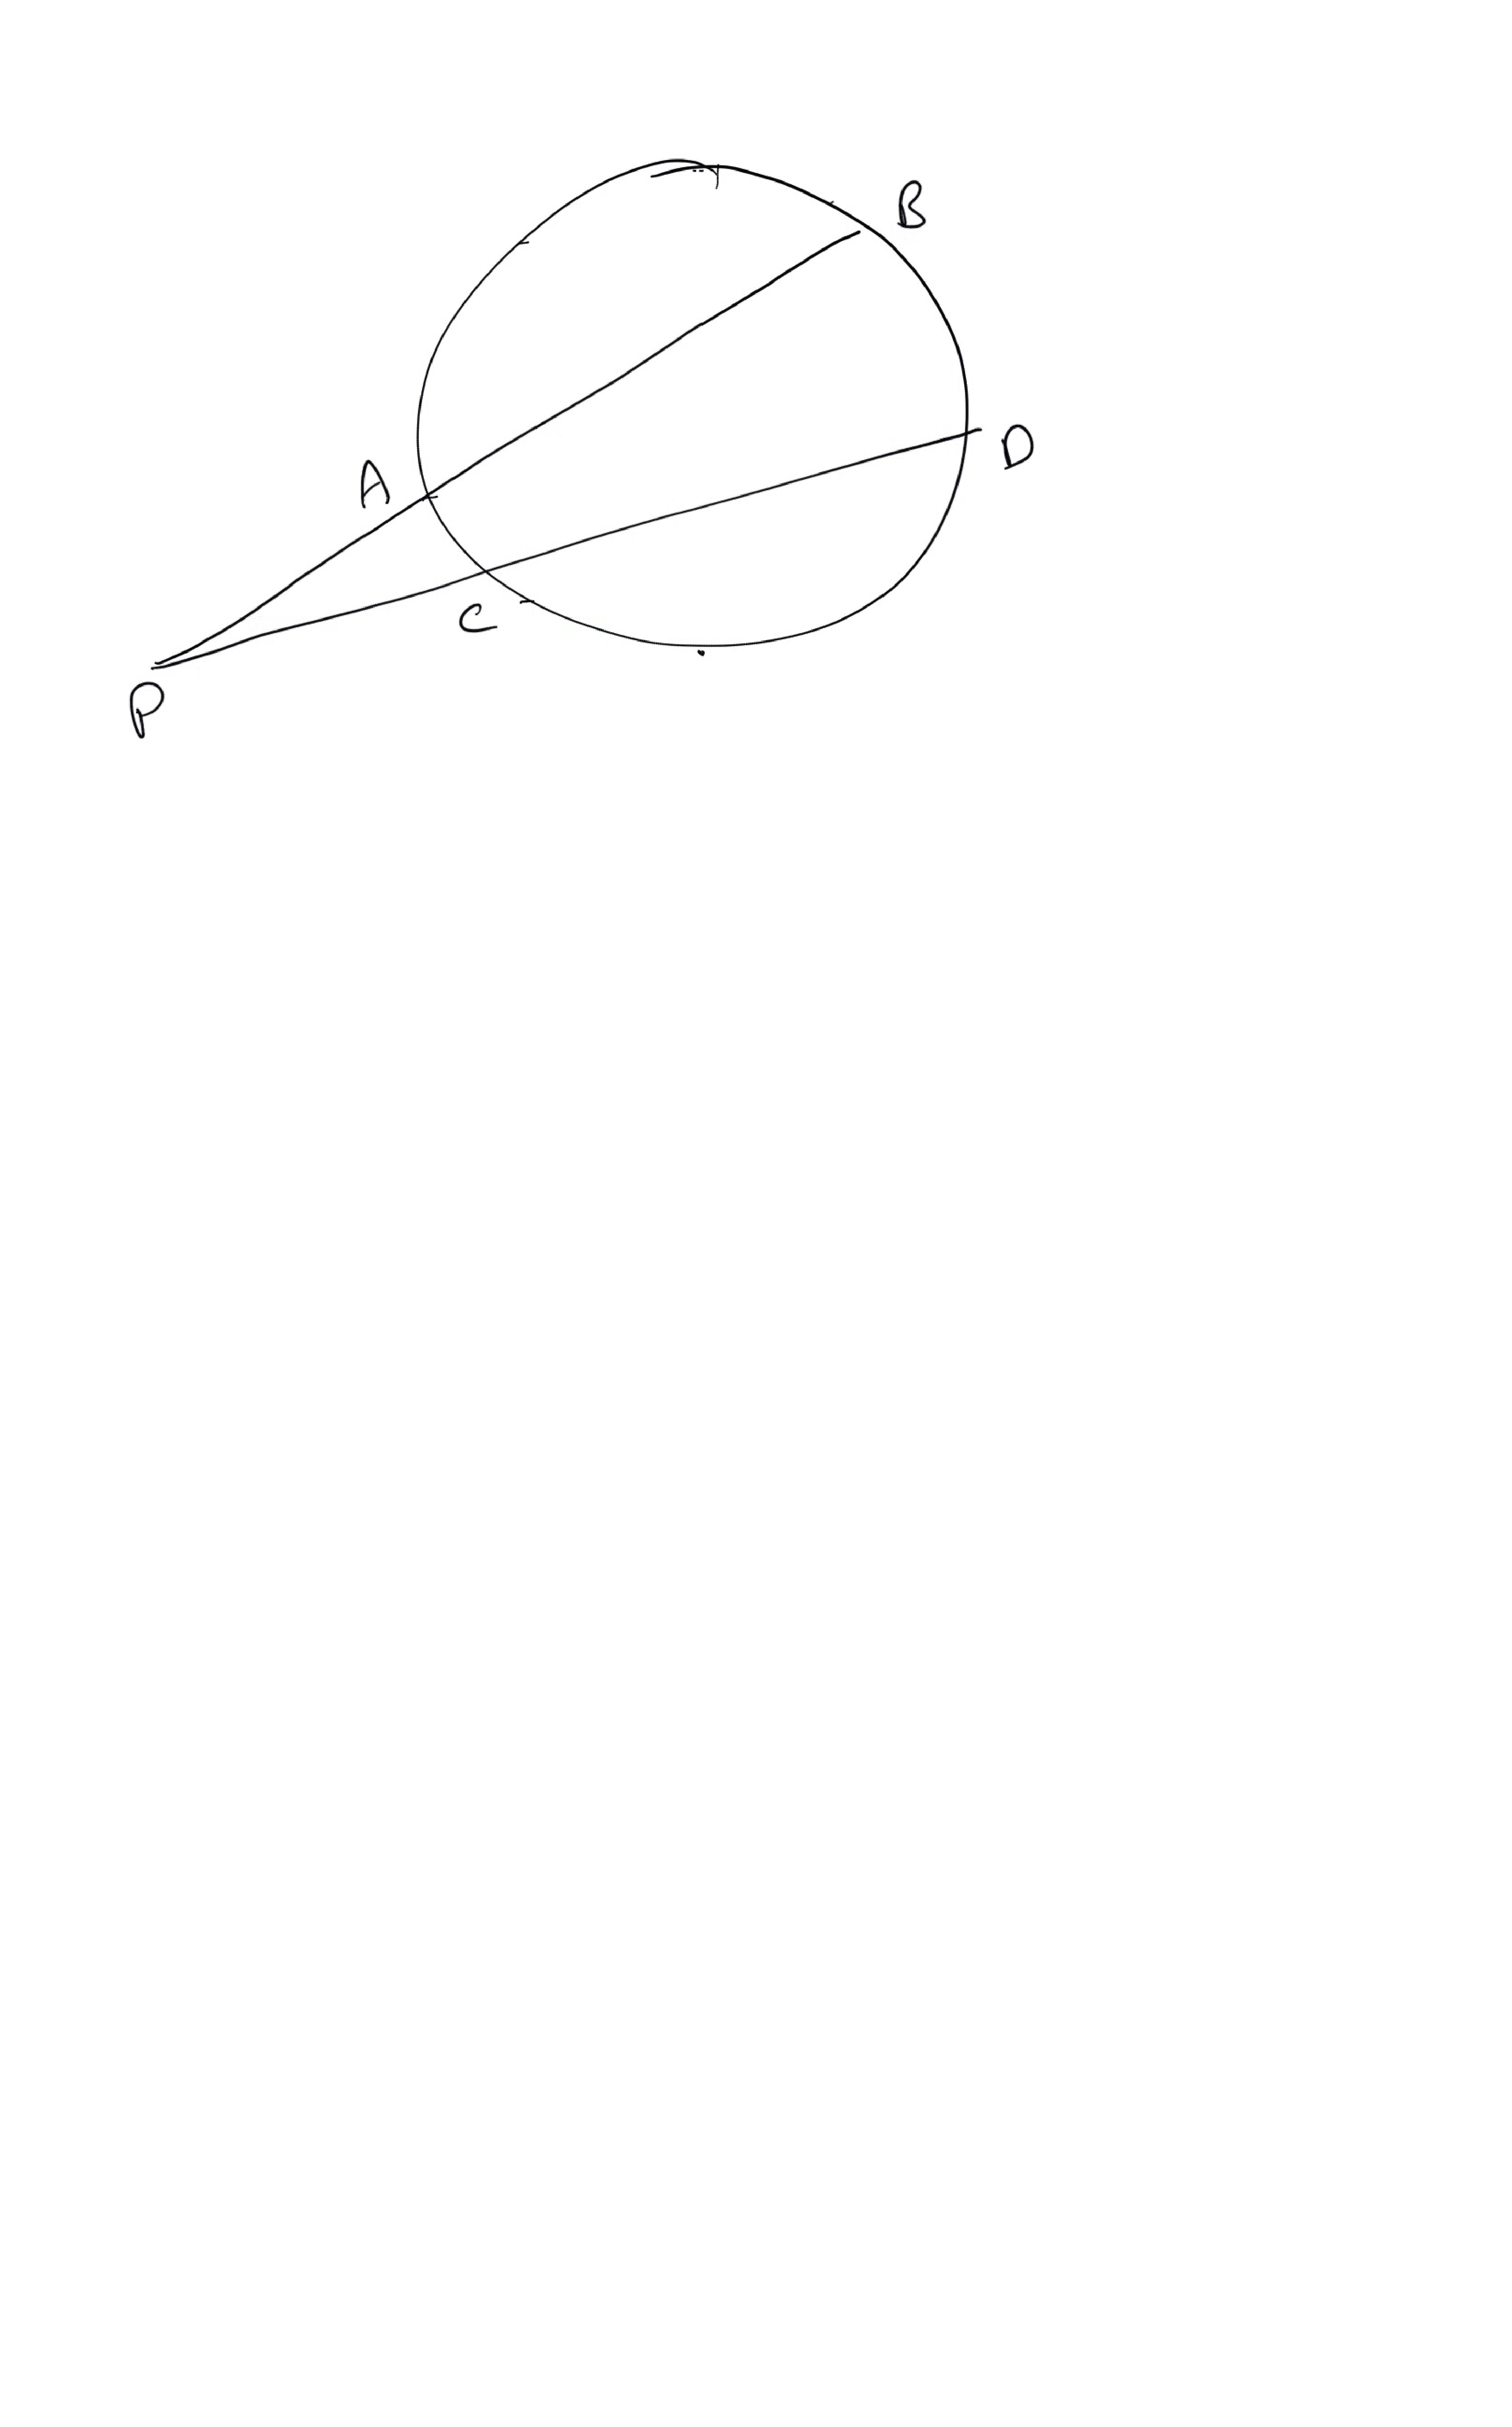
\includegraphics[width=\columnwidth]{./figs/ch4_chord_tangent_prod}
		%\vspace*{-10cm}
		\resizebox{\columnwidth}{!}{\begin{tikzpicture}
[scale =2,>=stealth,point/.style = {draw, circle, fill = black, inner sep = 1pt},]

\def\rad{2}
\coordinate [point, label={above: $O$ }] (O) at (0, 2);
\draw (O) circle (\rad);
\node (P) at (-5,0)[point,label=below :$P$] {};
\node (C) at (-1.65,0.9)[point,label=below :$C$] {};
\node (A) at (-2,2.3)[point,label=left :$A$] {};
\node (B) at (0.3,4)[point,label=above :$B$] {};
\node (D) at (2,2)[point,label=right :$D$] {};
\draw (C)--(D);
\draw (A)--(B);
\draw (A)--(P);
\draw (P)--(C);
\end{tikzpicture}}
	\end{center}
	\caption{$PA.PB = PC^2$.}
	\label{ch4_chord_tangent_prod}	
\end{figure}

\solution Draw a tangent and use the previous problem.
\end{enumerate}
